\section{Properties of Gaussian Distribution}
\begin{definition}[Multivariate Gaussian Distribution]
 We say $\bfx = (x_1,\cdots, x_n)$ has a multivariate Gaussian distribution if and only if every linear combination of its components has a (multivariate) Gaussian distribution. Formally,
$$
\bfx \sim \NN(\bfmu, \bfSigma) \Leftrightarrow A \bfx \sim \NN(A\bfmu, A \bfSigma A^\top), \ \forall A.
$$
\end{definition}

\begin{property}[Marginal Distribution]
	From the definition, any subset of random variables $\bfx' \subset \bfx$ are themselves normally distributed, and the mean and covariance is given by simply ignoring all elements that are not in $\bfx'$.
\end{property}

\begin{property}[Conditional Distribution]
	For a joint Gaussian distribution, if we given the values of some RVs $\bfy$, then the conditional distribution of the remaining RVs $\bfy_*$ is
	$$
	p(\bfy_* \mid \bfy) = \NN(\bfmu + \bfSigma_* \bfSigma_{**}^{-1}(\bfy_* - \bfmu_*), \bfSigma - \bfSigma_* \bfSigma_{**}^{-1}\bfSigma_*^\top ),
	$$
	where
	$$
\left[\begin{array}{c}
\bfy \\
\bfy_*
\end{array}\right] 
\sim \mathcal{N}\left(\left[\begin{array}{c}
\bfmu \\
\bfmu_*
\end{array}\right], \left[\begin{array}{cc}
\bfSigma & \bfSigma_* \\
\bfSigma_*^\top & \bfSigma_{**}
\end{array}\right]\right).
	$$
\end{property}
\begin{proof}
By definition, the conditional distribution for $\bfy_*$ given $\bfy$ is
\begin{align}
	p(\bfy_* \mid \bfy) & = \frac{p(\bfy, \bfy_*)}{p(\bfy)} \\
	& \propto \exp\left(-\frac{1}{2}\left[\bfy - \bfmu, \bfy_* - \bfmu_* \right]
\left[\begin{array}{cc}
\bfSigma & \bfSigma_* \\
\bfSigma_*^\top & \bfSigma_{**}
\end{array}\right]^{-1}
\left[\begin{array}{c}
\bfy - \bfmu \\
\bfy_* - \bfmu_*
\end{array}\right] 
\right)
\end{align}  
To get the inverse of covariance matrix, we need to diagonalize it,
\begin{align}
	\left[\begin{array}{cc}
\bfSigma & \bfSigma_* \\
\bfSigma_*^\top & \bfSigma_{**}
\end{array}\right] =
	\left[\begin{array}{cc}
\bmI & - \bfSigma_* \bfSigma_{**}^{-1} \\
0 & \bmI
\end{array}\right]^{-1}
	\left[\begin{array}{cc}
\bfSigma - \bfSigma_* \bfSigma_{**}^{-1} \bfSigma_*^{\top}  & 0 \\
0 & \bfSigma_{**}
\end{array}\right]
	\left[\begin{array}{cc}
\bmI & 0 \\
-\bfSigma_{**}^{-1}\bfSigma_*^\top & \bmI
\end{array}\right]^{-1}
\end{align}
Then, we get the inverse of the covariance matrix,
\begin{align}
	\left[\begin{array}{cc}
\bfSigma & \bfSigma_* \\
\bfSigma_*^\top & \bfSigma_{**}
\end{array}\right]^{-1} =
	\left[\begin{array}{cc}
\bmI & 0 \\
-\bfSigma_{**}^{-1}\bfSigma_*^\top & \bmI
\end{array}\right]
	\left[\begin{array}{cc}
(\bfSigma - \bfSigma_* \bfSigma_{**}^{-1} \bfSigma_*^{\top})^{-1}  & 0 \\
0 & \bfSigma_{**}^{-1}
\end{array}\right]
	\left[\begin{array}{cc}
\bmI & - \bfSigma_* \bfSigma_{**}^{-1} \\
0 & \bmI
\end{array}\right]
\end{align}
Plug it back into the conditional distribution, we get \marginpar{\footnotesize This can be viewed as the product of two Gaussians.}
\begin{align} &\left[\bfy - \bfmu, \bfy_* - \bfmu_* \right]
\left[\begin{array}{cc}
\bfSigma & \bfSigma_* \\
\bfSigma_*^\top & \bfSigma_{**}
\end{array}\right]^{-1}
\left[\begin{array}{c}
\bfy - \bfmu \\
\bfy_* - \bfmu_*
\end{array}\right] \\
=&\left(\bfy-\boldsymbol{\mu}_{1}-\bfSigma_{*}\bfSigma_{**}^{-1}\left(\bfy_*-\boldsymbol{\mu}_{2}\right)\right)^{\mathrm{T}}\left(\bfSigma_{11}-\bfSigma_{*}\bfSigma_{**}^{-1}\bfSigma_{21}\right)^{-1}\left(\bfy-\boldsymbol{\mu}_{1}-\bfSigma_{*}\bfSigma_{**}^{-1}\left(\bfy_*-\boldsymbol{\mu}_{2}\right)\right) \\
& +\left(\bfy_*-\boldsymbol{\mu}_{2}\right)^{\mathrm{T}}\bfSigma_{**}^{-1}\left(\bfy_*-\boldsymbol{\mu}_{2}\right)
\end{align} 
Therefore, the conditional distribution is 
\begin{equation}
	p(\bfy_* \mid \bfy) = \NN(\bfmu + \bfSigma_* \bfSigma_{**}^{-1}(\bfy_* - \bfmu_*), \bfSigma - \bfSigma_* \bfSigma_{**}^{-1}\bfSigma_*^\top )
\end{equation}
\end{proof}

\subsection{Prediction using Gaussian Processes}
\begin{definition}[Gaussian Process]
	A Gaussian Process (GP) is a (potentially infinite) collection of random variables (RV) such that the joint distribution of every finite subset of RVs is multivariate Gaussian:
	$$
	f \sim \mathrm{GP}(\mu(\bfx), K(\bfx, \bfx'))
	$$
where $\mu(\bfx): \cX \rightarrow \cX$ and $K(\bfx,\bfx'): \cX \times \cX \rightarrow \R $ are the mean and covariance function, respectively.
\end{definition}
Now, in order to model the predictive distribution $P(\bff_*\mid \bfx_*, D)$ we can use a Bayesian approach by using a GP prior: $p(\bff \mid \bfx)\sim \mathcal{N}(\mu, \bfSigma)$ and condition it on the training data $D$ to model the joint distribution of $\bff=f(\bfx)$ (vector of training observations) and $\bff_*=f(\bfx_*)$ (prediction at test input).


\begin{definition}[Predictive Distribution under Noise]
Let $y_i = f_i + \epsilon_i$, where $\EE[y_i] = 0$ and $\epsilon_i \sim \NN(0, \sigma^2)$. The predictive density $p(y_{n + 1} \mid \bfx_{n + 1}, \bfX, \bfy)$ for a new data point $\bfx_{n + 1}$ can be obtained analytically in Gaussian Process by deriving the joint distribution
$$
	p\left(\left[\begin{array}{c}
\mathbf{y} \\
y_{n+1}
\end{array}\right] \bigg|\ \bfx_{n+1}, \mathbf{X}, \sigma\right)=\mathcal{N}\left(\left[\begin{array}{c}
\mathbf{y} \\
y_{n+1}
\end{array}\right] \bigg|\ \mathbf{0},\left[\begin{array}{cc}
\mathbf{K} + \sigma^2 & \mathbf{k}_* \\
\mathbf{k}_*^{\top} & k + \sigma^2
\end{array}\right]\right)
$$	
where
$$
\bfK = \left[ K(\bfx_i, \bfx_j) \right]_{i=j=1}^{n}, \quad \mathbf{k}_* =  \left[K(\bfx_{n+1}, \bfx_i)\right]_{i=1}^{n},\quad k = K(\bfx_{n+1}, \bfx_{n+1}).
$$
\end{definition}
Using the conditional distribution of Gaussian, we have the closed-form solution of it,
\begin{equation}
	p(y_{n + 1} \mid \bfx_{n + 1}, \bfX, \bfy) = \NN(y_{n + 1} \mid \underbrace{\bfk^\top (\bfK + \sigma^2 \bfI)^{-1} \bfy}_\text{mean follows observations}, \underbrace{k -  \bfk^\top (\bfK + \sigma^2 \bfI)^{-1} \bfk}_\text{variance shrinks given more data}).
\end{equation}

\begin{property}[Model Selection in GP]
	A benefit of Gaussian Processes is that we can compute the marginal likelihood of the data given a model. This gives us a principled way of comparing different models.
\end{property}
\subsection{Kernels in Gaussian Processes}
Fig.~\ref{fig:ker1} and \ref{fig:ker2} give intuitive examples of the behavior of the kernels in GP. \footnote{Figures are taken from D. K. Duvenaud's Thesis: Automatic Model Construction with Gaussian Processes, Cambridge, 2014}
\newpage
\begin{figure}[h]
\center
	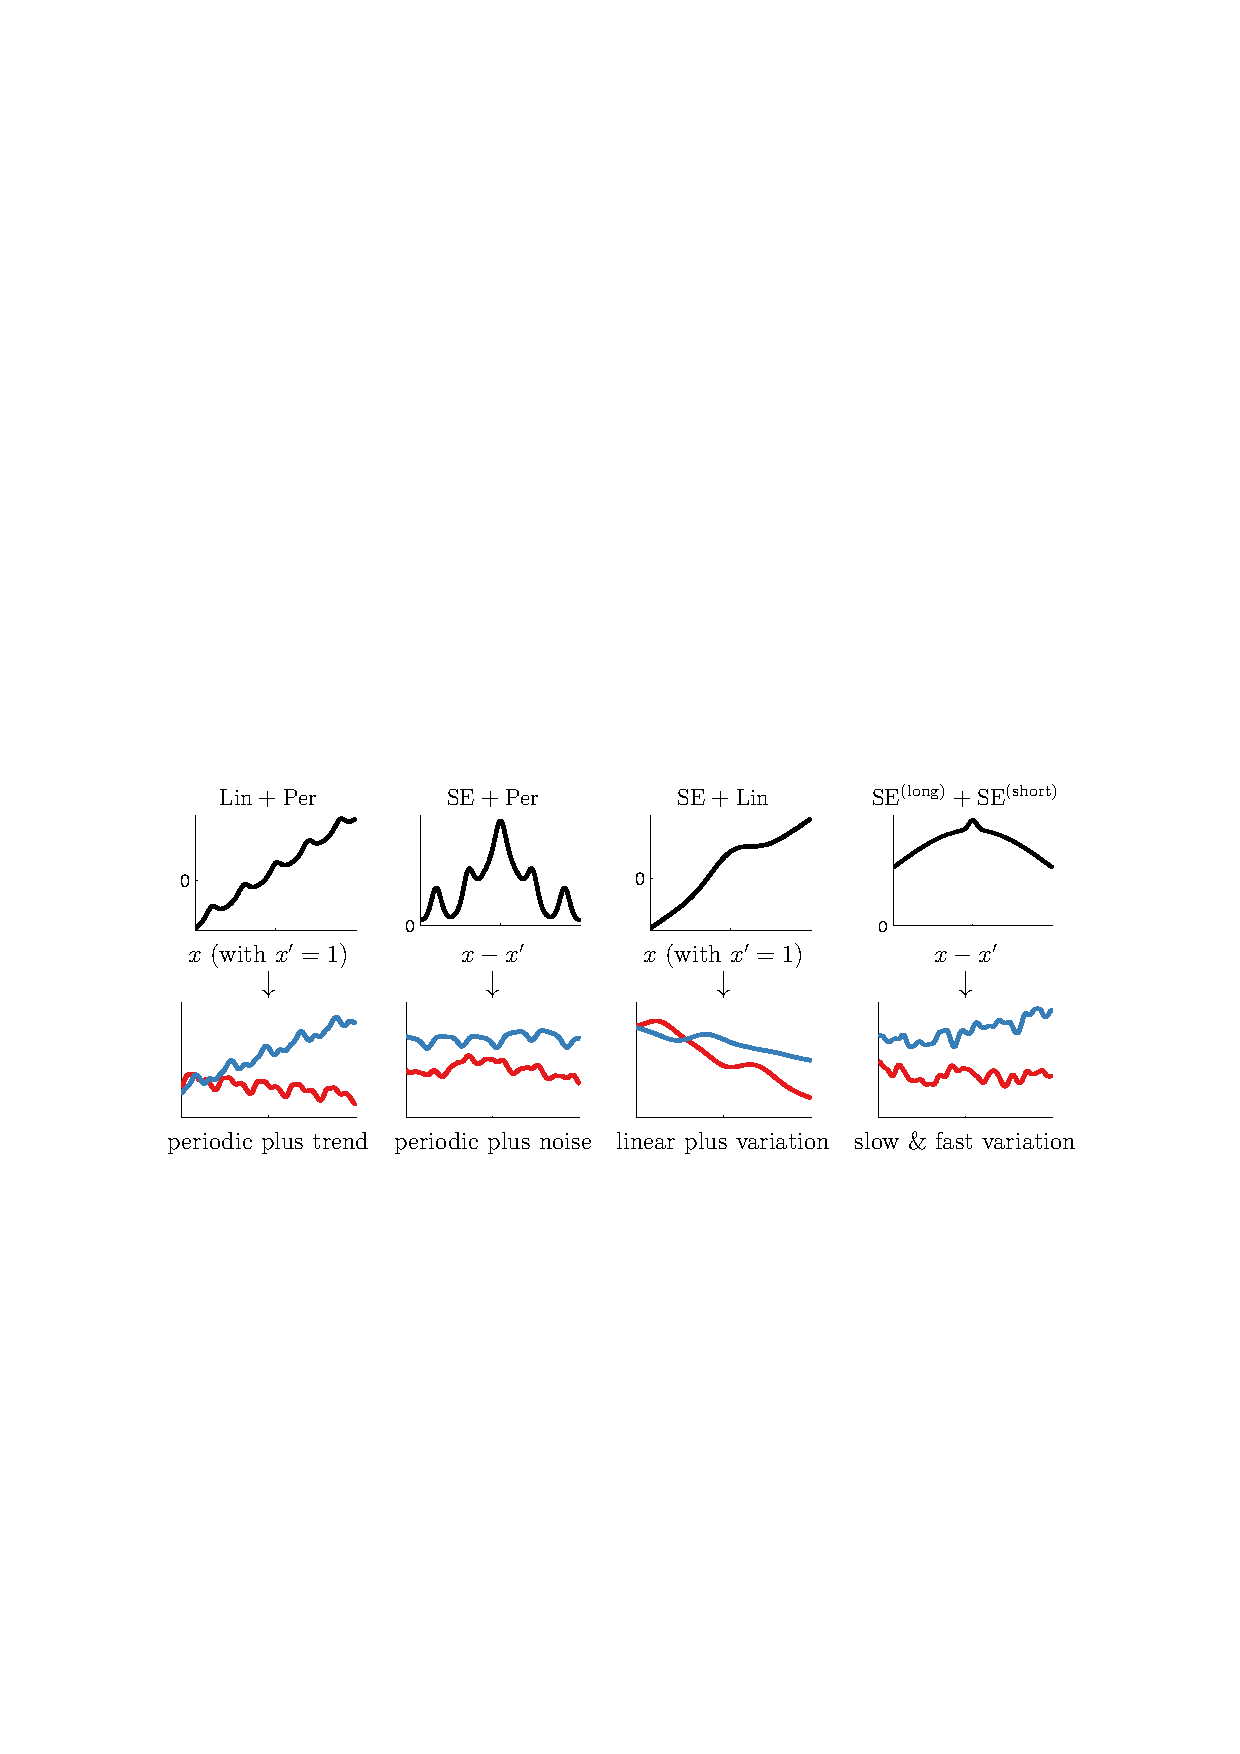
\includegraphics[width=0.95\textwidth]{figures/kernel1}
	\caption{Sum of different kernels \label{fig:ker1}}
\end{figure}
\vspace{0.5cm}
\begin{figure}[h]
\center
	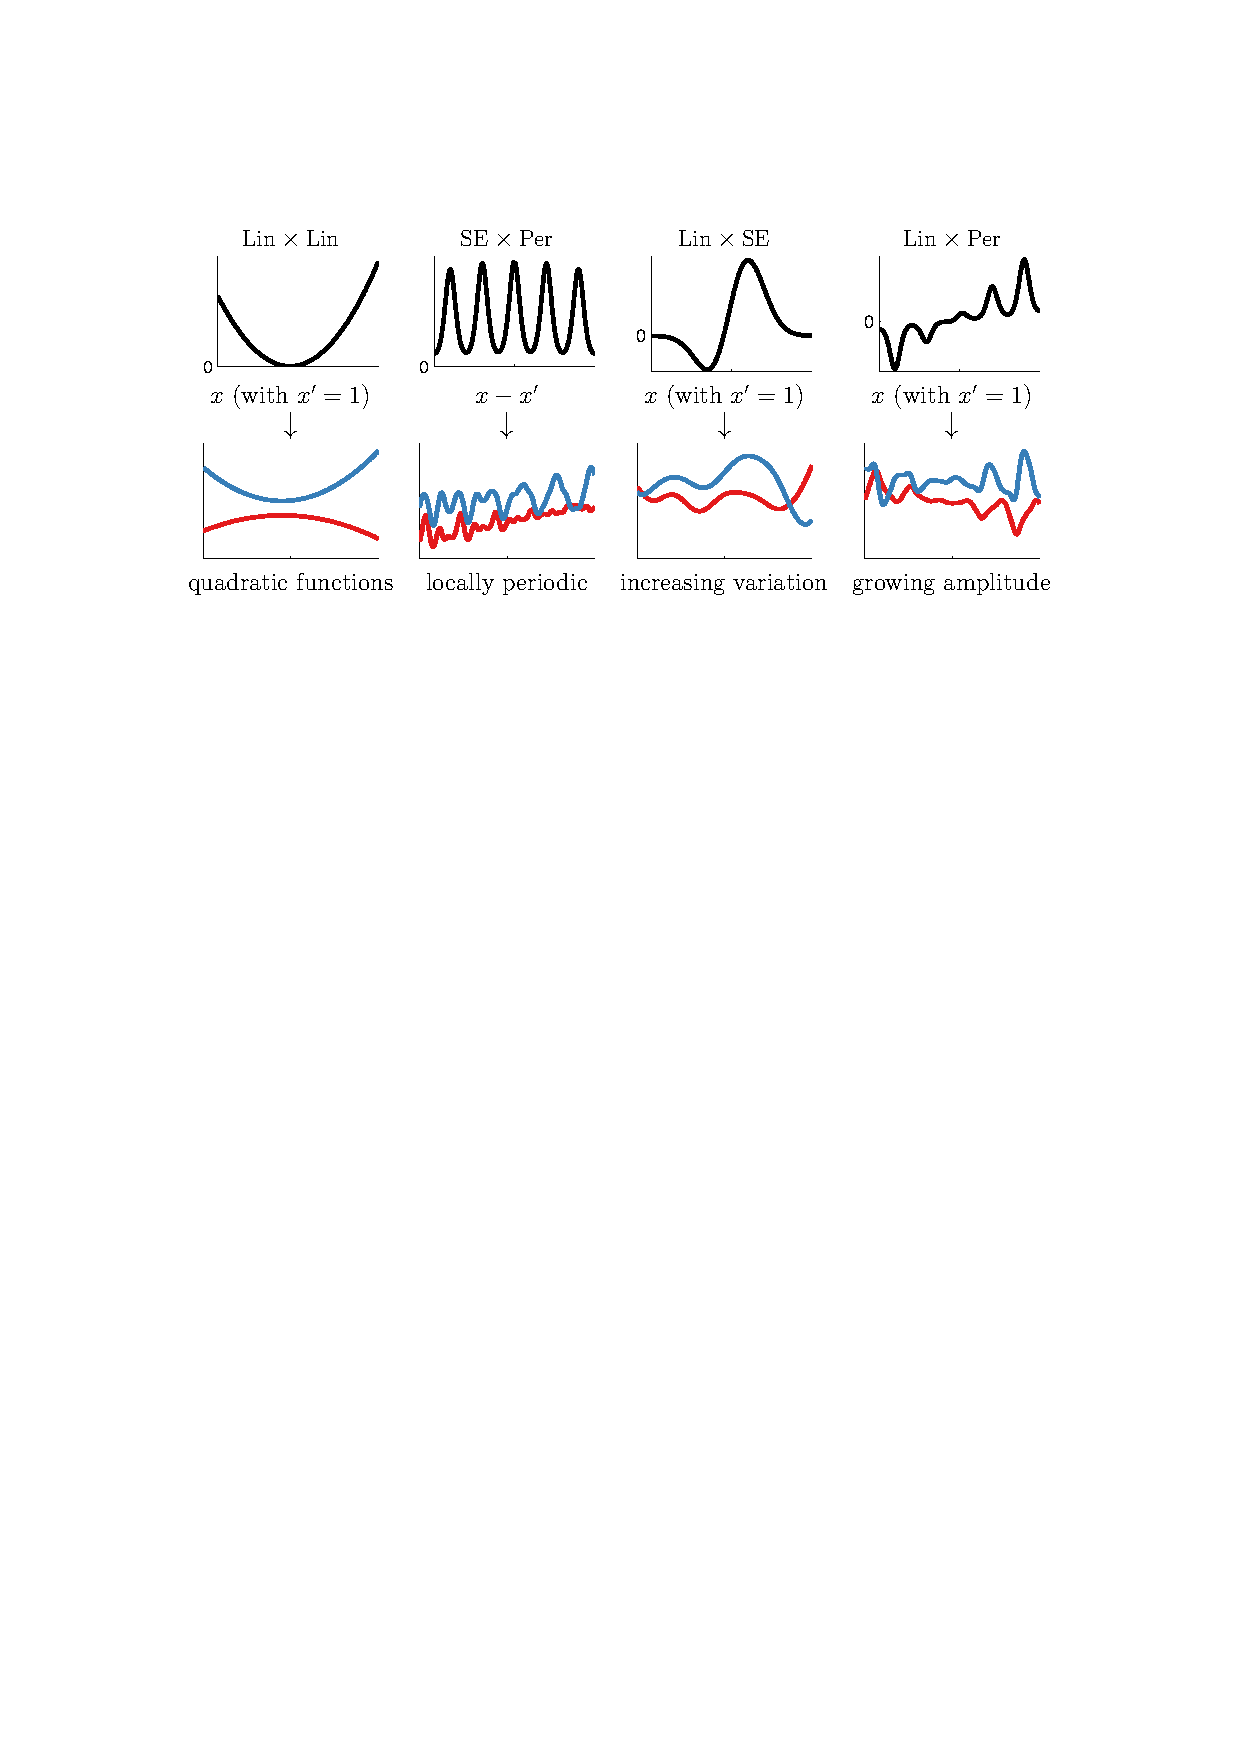
\includegraphics[width=0.95\textwidth]{figures/kernel2}
	\caption{Product of different kernels \label{fig:ker2}}
\end{figure}

